\documentclass{article}

\usepackage{graphicx}
\usepackage{refstyle}
\usepackage{subcaption}
\usepackage[table,xcdraw]{xcolor}

\def\RSfigtxt{Fig.\,}%
\def\RSfigstxt{Figs~}%
\def\RSFigtxt{Fig.\,}%
\def\RSFigstxt{Figs~}%

\begin{document}

\title{Intro to AI -- Final Paper Draft}
\author{
  William Horn\\
  \texttt{wbhorn@alaska.edu}
  \and
  Hal Dimarchi\\
  \texttt{hadimarchi@alaska.edu}
  \and
  Duane Shaffer\\
  \texttt{dlshaffer@alaska.edu}
  \and
  Kai Davids\\
  \texttt{kdavidsschell@alaska.edu}
}
\date{\today}
\maketitle

\section{Checkers}

For the beginning of the project, we created a program by making a
move generator and a random move selector. The move generator was used to get
valid moves on an 8x8 checkers board at any point in the game. Internally this
corresponded to a list of characters of size 32 because half of the 64 spaces
can never be visited. The move selector takes moves from the generator, if a
jump is present it must be taken. This left us with creating players that could
use the board and move generator to play a checkers game.

The game itself has two players, red and black. The players keep track of their pieces and what
those pieces can do. The move generators gives hypothetically valid moves that
the player class uses when selecting a move, initially the moves were picked at
random. Further improvements on the checkers program were to create a piece
count evaluator that chose moves by traversing the search tree of possible
moves (see minimax) and picking the move that lead to the best outcome. The
heuristic used to evaluate was to sum up the pieces on the board for each
player, giving a larger weight to kings, and taking the difference between the
two players. This ended up being quite a good heuristic for evaluating moves
and lead to more intelligent move selection.

\figref{game} and Table \ref{table:moves-jumps}. show the checkers game running along with the GUI.
The table shows all the valid possible moves and jumps at the point of the
screenshot. The numbers in the table correspond to the location in \figref{board-key}.

\section{Searching}

Searching is done to select the move that will have the highest chance of
leading to a win for the searching player.  This can be done using either a
breadth first search (BFS) or a depth first search (DFS). To save on memory
we used a DFS.

\subsection{Minimax}

In minimax searching the program starts with all moves currently available to
it, and expands them, by assuming they have been taken, and then recursing on
the resulting available moves to a chosen depth. The search alternates between
choosing the move that will result in the best case scenario for the searching
player, and the move that will result in the worst case scenario for the
searching player (assuming that the enemy will choose those moves). Once it has
reached the max depth or the game is over, it performs an evaluation of the
state of the board and returns it. The program chooses the move that leads to
the sub-tree with the best possible result.

\subsubsection{Statistics (Depth 5)}
\begin{itemize}
	\item Boards expanded per move: 6121.88
	\item Board evaluation functions called: 26,518.45
	\item Inner vs. leaf nodes: 0.19
\end{itemize}

\subsection{Alpha-Beta}

Alpha-beta pruning is an improvement on the minimax searching algorithm that
removes branches that are unlikely to be useful. It does so by keeping track of
2 values, alpha, the best explored path to the root for the maximiser, and
beta, the best explored path to the root for the minimizer. When expanding
nodes and looking at paths for the maximizer, if the program finds an option
that will allow the maximizer to achieve a higher value path back to the root
than a path already explored then all children of the parent of that leaf node
can be pruned, because the minimizer presumably will not choose that option.
Because this means whole subtrees don’t need to be fully expanded, it allows
for either deeper searches  or for a more computationally intensive board
evaluation function. The graphs in \figref{ab-v-mm} show the number of nodes expanded for
minimax with and without alpha-beta pruning at different depths.

\subsubsection{Statistics (Depth 5)}
\begin{itemize}
	\item Boards expanded per move: 1036.2
	\item Board evaluation functions called: 1605.80
	\item Inner vs. leaf nodes: 0.39
    \item Nodes pruned: 29998.33 (inner and leaf)
\end{itemize}

\begin{figure}[ht!]
    \centering
    \begin{subfigure}[b]{0.4\linewidth}
        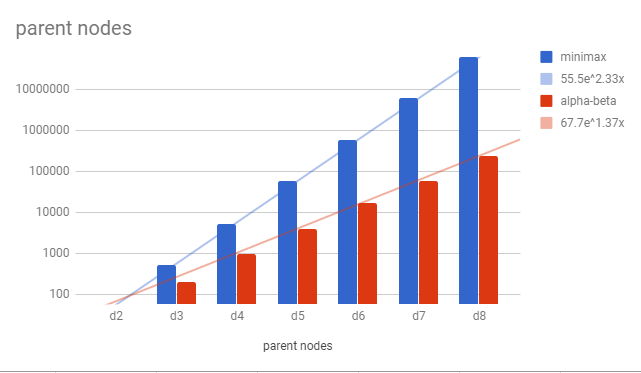
\includegraphics[width=\linewidth]{images/parent-nodes-abvmm.png}
        \caption{parent (inner) nodes evaluated in minimax vs alpha-beta}
    \end{subfigure}
    \begin{subfigure}[b]{0.4\linewidth}
        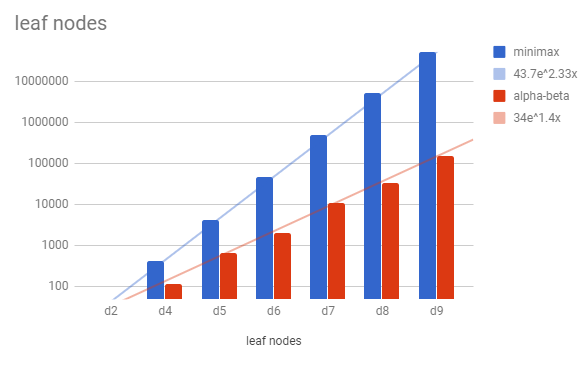
\includegraphics[width=\linewidth]{images/leaf-nodes-abvmm.png}
        \caption{Comparing leaf nodes evaluated in minimax vs alpha-beta}
    \end{subfigure}

    \caption{Comparing minimax and alpha-beta search methods.}
    \label{fig:ab-v-mm}
\end{figure}

\subsection{Implementation}

To implement alpha-beta the same checkers-game class used to play a regular
game was used to search through possible future moves and jumps. It was implimented
using a recursive DFS search \figref{ab-code}.

\begin{figure*}
    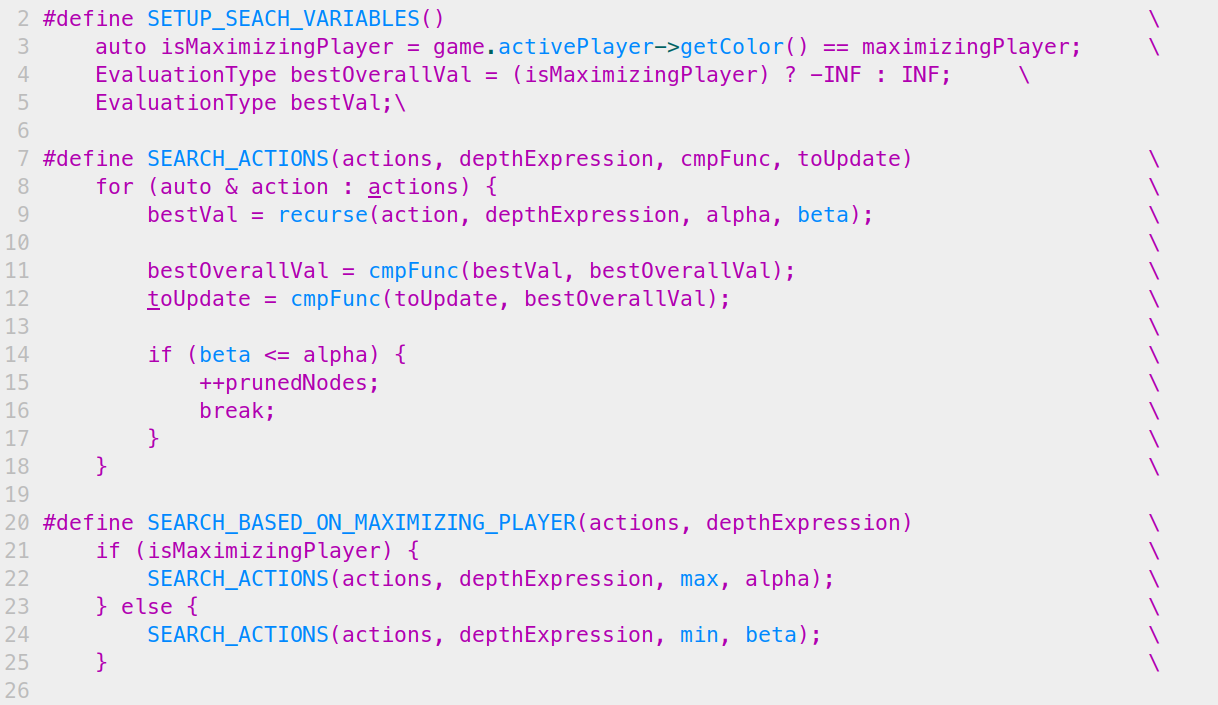
\includegraphics[width=\linewidth]{images/alpha-beta-code.png}
    \caption{alpha beta c++ implimentation}
    \label{fig:ab-code}
\end{figure*}

Preprocessor macros are used for two reasons (\figref{ab-code}), the best way to write the loop
through all the action (moves/jumps) is to take the isMaximizingPlayer check
out of the loop, which means writing it twice and because instead of recursing
on boards, move and jumps are used to recures on. This means two very similar
function because they are different types.

In the SEARCH\textunderscore{}ON\textunderscore{}MAXIMIZING\textunderscore{}PLAYER (\figref{ab-code})
macro the actions is either a list of valid
moves or jumps depending on what function the macro is expanded in. The
depthExpression is either n or n - 1. This is done because when recursing on
jumps or multi jumps the branch factor is low.

Time permitting this version
will be switched to a version that recuses on boards so that iterative
deepening search is easier to implement. Currently when a piece makes a
multijump this search is called multiple times for each jump, instead of once
for the whole jump. Recusing on a board would negate this because the entire
multijump would be counted as one move.

\section{Neural Networks}

A basic feed forward neural network (NN) consists of an input layer
with a variable amount of hidden layers and an output layer. All of the layers
consist of nodes and these nodes are connected from layer to layer. The input
layer consists of the data being given to the network that has been formatted
to numbers. Each node in the next layer has an amount of weights equal to the
number of input nodes. Further nodes have a number of weights equal the size of
the layer before them. To calculate a node, multiply each of the previous layer
nodes by their associated weights, add them together, and multiply by an
activator function. This process is repeated for each layer, causing the values
of each node to feed farther forward in the network culminating in a final
value for the output. \figref{nn-code} shows the c++ that impliments this technique.
The performance of the NN code is measured in board evaluations per
second (BPS).

\begin{figure}
    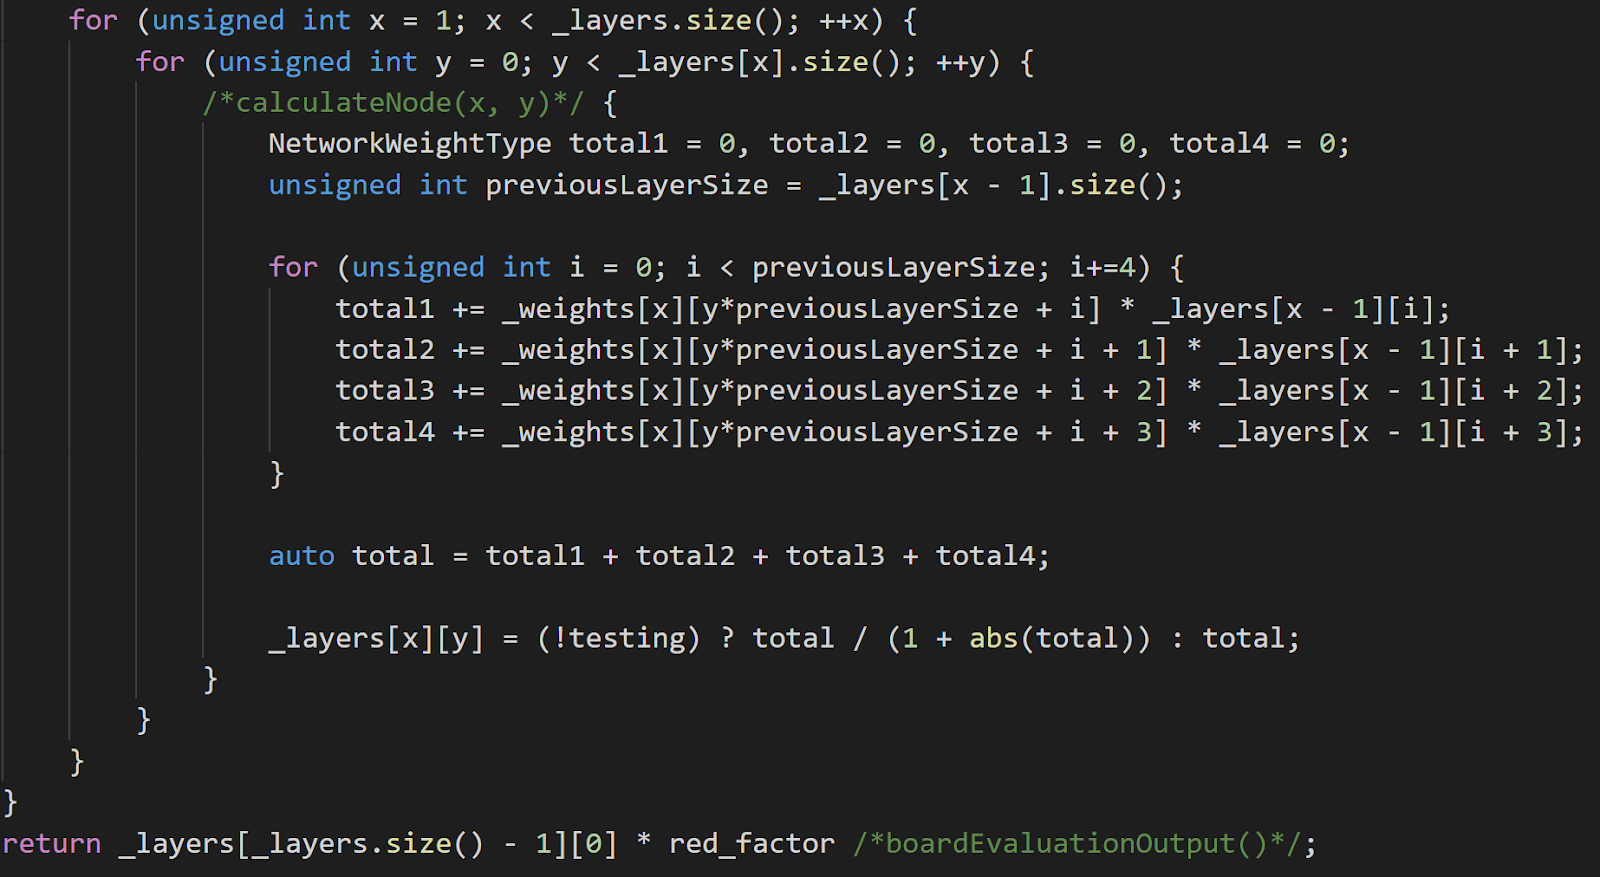
\includegraphics[width=\linewidth]{images/nn-code.png}
    \caption{Neural network c++ code}
    \label{fig:nn-code}
\end{figure}

\subsection{Timing}

\begin{itemize}
    \item Blondie24 (32-40-10-1)   : 879,833 bps
    \item Larger    (32-1000-100-1): 13762.5 bps
\end{itemize}

\subsection{Evolution (3-10-1 Topology)}

\figref{3-10-1-before} shows the contents of a random
NN following the given topology. \figref{3-10-1-after} shows values in the offspring from the
parent in previous image (the evolved network).

In order to show that our offspring is correct, a
histogram was made of the change in weight value between parent and offspring. The
changes show a model Gaussian distribution. The evolution process was simply following formulas
given. Between graphical representation of the change in weights and visual
confirmation of viable values for other parameters of the network. This proves that
the evolution process was happening properly.

To prove that the Gaussian pseudo-random number generator is absolutely correct, \figref{gaussian-2}
a histogram of 1000 numbers was made and this confirmed that our generator was in fact Gaussian.

\section{Evolutionary Learning}

There are several design considerations for evolutionary
learning that varies between the members of our group. For the trial section of
our project, we just used elements from Blondie24’s experiment. This includes a
NN topology of 32-40-10-1, a population size of 30, and a survival of the
fittest method of evolution where the best half of the networks create
offspring, evolve, and replace the lower half of the networks. Not all of our
members have decided on the topology they want to evolve but one experimental
topology is 32-1000-1 with a population size of 100. All networks follow the
Blondie24 method of evolution.

Networks are matched up against each other with
every network playing 5 games as red side versus a random network on black
side. Winners get one point and losers lose 2. Nothing happens to a NNs
performance when a draw occurs. These games compose a points based tournament
that allows networks to be sorted based on their performance.

\subsection{Statistics}

One of the testing topologies used was a 32-200-20 NN. For this tourament we only
played 3 games per match and ran at a alpha-beta search depth of 6. The tournaments
were run on a Digital Ocean cloud server running with 2 vCPUs. Threading was done
on a per game level so generations could be done faster. The time below is normalized for
1 vCPU and does not taken into account the time benefits from threading at a generation
level.

\begin{itemize}
    \item Time For a Game       : 13.53 seconds
    \item Time For a Generation : 1217.04 seconds
    \item Generations Per Day   : 71.00 gpd
\end{itemize}

\begin{figure}
    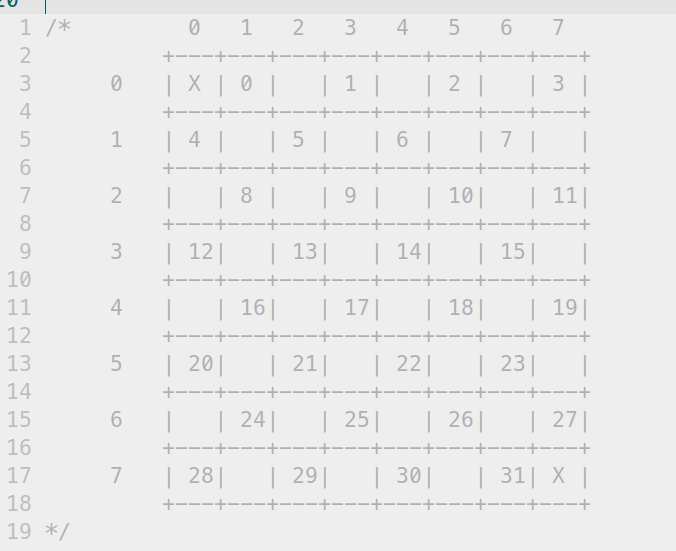
\includegraphics[width=\linewidth]{images/board-key.png}
    \caption{Numbering system used to store board states internally.}
    \label{fig:board-key}
\end{figure}

\begin{figure}
\begin{tabular}{cc}
  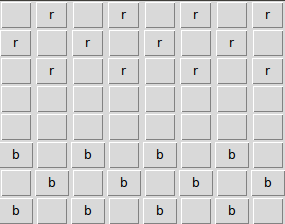
\includegraphics[width=65mm]{images/game-start.png} &   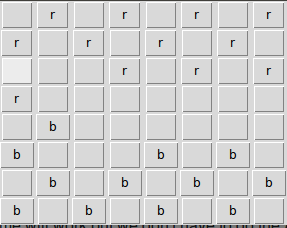
\includegraphics[width=65mm]{images/game-1.png} \\
(a) beginning & (b) midgame \\[6pt]
 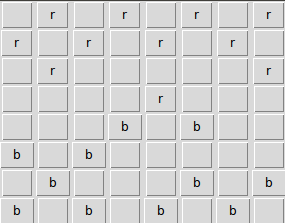
\includegraphics[width=65mm]{images/game-2.png} &   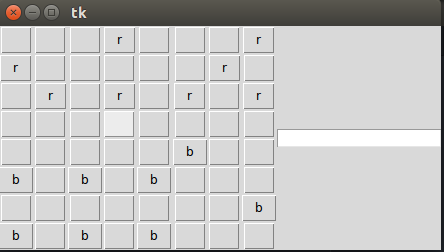
\includegraphics[width=65mm]{images/game-3.png} \\
(c) midgame & (d) midgame \\[6pt]
 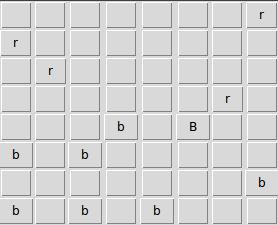
\includegraphics[width=65mm]{images/game-4.png} &   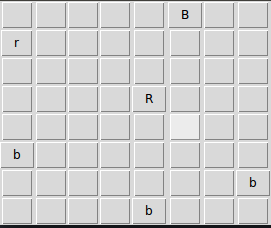
\includegraphics[width=65mm]{images/game-5.png} \\
 (e) midgame & (f) endgame \\[6pt]
\end{tabular}
\caption{Screenshots of the GUI at different stages in the game.}
\label{fig:game}
\end{figure}

\begin{table}[]
\centering
\caption{All possible valid moves and jumps for the gui screenshots in \figref{game}}
\label{table:moves-jumps}
\begin{tabular}{|lllllllll|}
\hline
\multicolumn{9}{|l|}{\textbf{Move/Jump Generator Output For Black}}                                                                                                                                                                                                                                                                                                  \\ \hline
\multicolumn{3}{|l|}{\textbf{Fig 1a.}}                                                                                 & \multicolumn{3}{l|}{\textbf{Fig 1b.}}                                                                                       & \multicolumn{3}{l|}{\textbf{Fig 1c.}}                                                                         \\ \hline
\multicolumn{1}{|l|}{\textbf{Moves}}           & \multicolumn{1}{l|}{\textbf{From}} & \multicolumn{1}{l|}{\textbf{To}} & \multicolumn{1}{l|}{\textbf{Moves}}           & \multicolumn{1}{l|}{\textbf{From}} & \multicolumn{1}{l|}{\textbf{To}}       & \multicolumn{1}{l|}{\textbf{Jumps}}           & \multicolumn{1}{l|}{\textbf{From}} & \textbf{Thru, To}        \\ \hline
\multicolumn{1}{|l|}{\cellcolor[HTML]{C0C0C0}} & \multicolumn{1}{l|}{20}            & \multicolumn{1}{l|}{16}          & \multicolumn{1}{l|}{\cellcolor[HTML]{C0C0C0}} & \multicolumn{1}{l|}{16}            & \multicolumn{1}{l|}{13}                & \multicolumn{1}{l|}{\cellcolor[HTML]{C0C0C0}} & \multicolumn{1}{l|}{18}            & (14, 9)                  \\ \cline{7-9}
\multicolumn{1}{|l|}{\cellcolor[HTML]{C0C0C0}} & \multicolumn{1}{l|}{21}            & \multicolumn{1}{l|}{16, 17}      & \multicolumn{1}{l|}{\cellcolor[HTML]{C0C0C0}} & \multicolumn{1}{l|}{22}            & \multicolumn{1}{l|}{17, 18}            & \multicolumn{1}{l|}{\textbf{Moves}}           & \multicolumn{1}{l|}{\textbf{From}} & \textbf{To}              \\ \cline{7-9}
\multicolumn{1}{|l|}{\cellcolor[HTML]{C0C0C0}} & \multicolumn{1}{l|}{22}            & \multicolumn{1}{l|}{17, 18}      & \multicolumn{1}{l|}{\cellcolor[HTML]{C0C0C0}} & \multicolumn{1}{l|}{23}            & \multicolumn{1}{l|}{18, 19}            & \multicolumn{1}{l|}{\cellcolor[HTML]{C0C0C0}} & \multicolumn{1}{l|}{16}            & 12, 13                   \\
\multicolumn{1}{|l|}{\cellcolor[HTML]{C0C0C0}} & \multicolumn{1}{l|}{23}            & \multicolumn{1}{l|}{18, 19}      & \multicolumn{1}{l|}{\cellcolor[HTML]{C0C0C0}} & \multicolumn{1}{l|}{24}            & \multicolumn{1}{l|}{21}                & \multicolumn{1}{l|}{\cellcolor[HTML]{C0C0C0}} & \multicolumn{1}{l|}{18}            & 15                       \\ \cline{2-3}
\cellcolor[HTML]{C0C0C0}                       & \cellcolor[HTML]{C0C0C0}           & \cellcolor[HTML]{C0C0C0}         & \multicolumn{1}{l|}{\cellcolor[HTML]{C0C0C0}} & \multicolumn{1}{l|}{25}            & \multicolumn{1}{l|}{21}                & \multicolumn{1}{l|}{\cellcolor[HTML]{C0C0C0}} & \multicolumn{1}{l|}{23}            & 19                       \\ \cline{5-6}
\cellcolor[HTML]{C0C0C0}                       & \cellcolor[HTML]{C0C0C0}           & \cellcolor[HTML]{C0C0C0}         & \cellcolor[HTML]{C0C0C0}                      & \cellcolor[HTML]{C0C0C0}           & \cellcolor[HTML]{C0C0C0}               & \multicolumn{1}{l|}{\cellcolor[HTML]{C0C0C0}} & \multicolumn{1}{l|}{24}            & 21                       \\
\cellcolor[HTML]{C0C0C0}                       & \cellcolor[HTML]{C0C0C0}           & \cellcolor[HTML]{C0C0C0}         & \cellcolor[HTML]{C0C0C0}                      & \cellcolor[HTML]{C0C0C0}           & \cellcolor[HTML]{C0C0C0}               & \multicolumn{1}{l|}{\cellcolor[HTML]{C0C0C0}} & \multicolumn{1}{l|}{26}            & 22                       \\
\cellcolor[HTML]{C0C0C0}                       & \cellcolor[HTML]{C0C0C0}           & \cellcolor[HTML]{C0C0C0}         & \cellcolor[HTML]{C0C0C0}                      & \cellcolor[HTML]{C0C0C0}           & \cellcolor[HTML]{C0C0C0}               & \multicolumn{1}{l|}{\cellcolor[HTML]{C0C0C0}} & \multicolumn{1}{l|}{29}            & 25                       \\
\cellcolor[HTML]{C0C0C0}                       & \cellcolor[HTML]{C0C0C0}           & \cellcolor[HTML]{C0C0C0}         & \cellcolor[HTML]{C0C0C0}                      & \cellcolor[HTML]{C0C0C0}           & \cellcolor[HTML]{C0C0C0}               & \multicolumn{1}{l|}{\cellcolor[HTML]{C0C0C0}} & \multicolumn{1}{l|}{30}            & 25                       \\ \hline
\multicolumn{3}{|l|}{\textbf{Fig 1d.}}                                                                                 & \multicolumn{3}{l|}{\textbf{Fig 1e.}}                                                                                       & \multicolumn{3}{l|}{\textbf{Fig 1f.}}                                                                         \\ \hline
\multicolumn{1}{|l|}{\textbf{Moves}}           & \multicolumn{1}{l|}{\textbf{From}} & \multicolumn{1}{l|}{\textbf{To}} & \multicolumn{1}{l|}{\textbf{Jumps}}           & \multicolumn{1}{l|}{\textbf{From}} & \multicolumn{1}{l|}{\textbf{Thru, To}} & \multicolumn{1}{l|}{\textbf{Moves}}           & \multicolumn{1}{l|}{\textbf{From}} & \textbf{To}              \\ \hline
\multicolumn{1}{|l|}{\cellcolor[HTML]{C0C0C0}} & \multicolumn{1}{l|}{18}            & \multicolumn{1}{l|}{14, 15}      & \multicolumn{1}{l|}{\cellcolor[HTML]{C0C0C0}} & \multicolumn{1}{l|}{18}            & \multicolumn{1}{l|}{(15, 11)}          & \multicolumn{1}{l|}{\cellcolor[HTML]{C0C0C0}} & \multicolumn{1}{l|}{2}             & 6, 7                     \\ \cline{4-6}
\multicolumn{1}{|l|}{\cellcolor[HTML]{C0C0C0}} & \multicolumn{1}{l|}{20}            & \multicolumn{1}{l|}{16}          & \multicolumn{1}{l|}{\textbf{Moves}}           & \multicolumn{1}{l|}{\textbf{From}} & \multicolumn{1}{l|}{\textbf{To}}       & \multicolumn{1}{l|}{\cellcolor[HTML]{C0C0C0}} & \multicolumn{1}{l|}{20}            & 16                       \\ \cline{4-6}
\multicolumn{1}{|l|}{\cellcolor[HTML]{C0C0C0}} & \multicolumn{1}{l|}{21}            & \multicolumn{1}{l|}{16, 17}      & \multicolumn{1}{l|}{\cellcolor[HTML]{C0C0C0}} & 17                                 & \multicolumn{1}{l|}{13, 14}            & \multicolumn{1}{l|}{\cellcolor[HTML]{C0C0C0}} & \multicolumn{1}{l|}{27}            & 23                       \\
\multicolumn{1}{|l|}{\cellcolor[HTML]{C0C0C0}} & \multicolumn{1}{l|}{22}            & \multicolumn{1}{l|}{17}          & \multicolumn{1}{l|}{\cellcolor[HTML]{C0C0C0}} & 18                                 & \multicolumn{1}{l|}{14, 22, 23}        & \multicolumn{1}{l|}{\cellcolor[HTML]{C0C0C0}} & \multicolumn{1}{l|}{30}            & 25, 26                   \\ \cline{8-9}
\multicolumn{1}{|l|}{\cellcolor[HTML]{C0C0C0}} & \multicolumn{1}{l|}{27}            & \multicolumn{1}{l|}{23}          & \multicolumn{1}{l|}{\cellcolor[HTML]{C0C0C0}} & 20                                 & \multicolumn{1}{l|}{16}                & \cellcolor[HTML]{C0C0C0}                      & \cellcolor[HTML]{C0C0C0}           & \cellcolor[HTML]{C0C0C0} \\
\multicolumn{1}{|l|}{\cellcolor[HTML]{C0C0C0}} & \multicolumn{1}{l|}{28}            & \multicolumn{1}{l|}{24}          & \multicolumn{1}{l|}{\cellcolor[HTML]{C0C0C0}} & 21                                 & \multicolumn{1}{l|}{16}                & \cellcolor[HTML]{C0C0C0}                      & \cellcolor[HTML]{C0C0C0}           & \cellcolor[HTML]{C0C0C0} \\
\multicolumn{1}{|l|}{\cellcolor[HTML]{C0C0C0}} & \multicolumn{1}{l|}{29}            & \multicolumn{1}{l|}{24, 25}      & \multicolumn{1}{l|}{\cellcolor[HTML]{C0C0C0}} & 27                                 & \multicolumn{1}{l|}{23}                & \cellcolor[HTML]{C0C0C0}                      & \cellcolor[HTML]{C0C0C0}           & \cellcolor[HTML]{C0C0C0} \\
\multicolumn{1}{|l|}{\cellcolor[HTML]{C0C0C0}} & \multicolumn{1}{l|}{30}            & \multicolumn{1}{l|}{25, 26}      & \multicolumn{1}{l|}{\cellcolor[HTML]{C0C0C0}} & 28                                 & \multicolumn{1}{l|}{24}                & \cellcolor[HTML]{C0C0C0}                      & \cellcolor[HTML]{C0C0C0}           & \cellcolor[HTML]{C0C0C0} \\ \cline{2-3}
\cellcolor[HTML]{C0C0C0}                       & \cellcolor[HTML]{C0C0C0}           & \cellcolor[HTML]{C0C0C0}         & \multicolumn{1}{l|}{\cellcolor[HTML]{C0C0C0}} & 29                                 & \multicolumn{1}{l|}{24, 25}            & \cellcolor[HTML]{C0C0C0}                      & \cellcolor[HTML]{C0C0C0}           & \cellcolor[HTML]{C0C0C0} \\
\cellcolor[HTML]{C0C0C0}                       & \cellcolor[HTML]{C0C0C0}           & \cellcolor[HTML]{C0C0C0}         & \multicolumn{1}{l|}{\cellcolor[HTML]{C0C0C0}} & 30                                 & \multicolumn{1}{l|}{25, 26}            & \cellcolor[HTML]{C0C0C0}                      & \cellcolor[HTML]{C0C0C0}           & \cellcolor[HTML]{C0C0C0} \\ \hline
\end{tabular}
\end{table}

\begin{figure}
    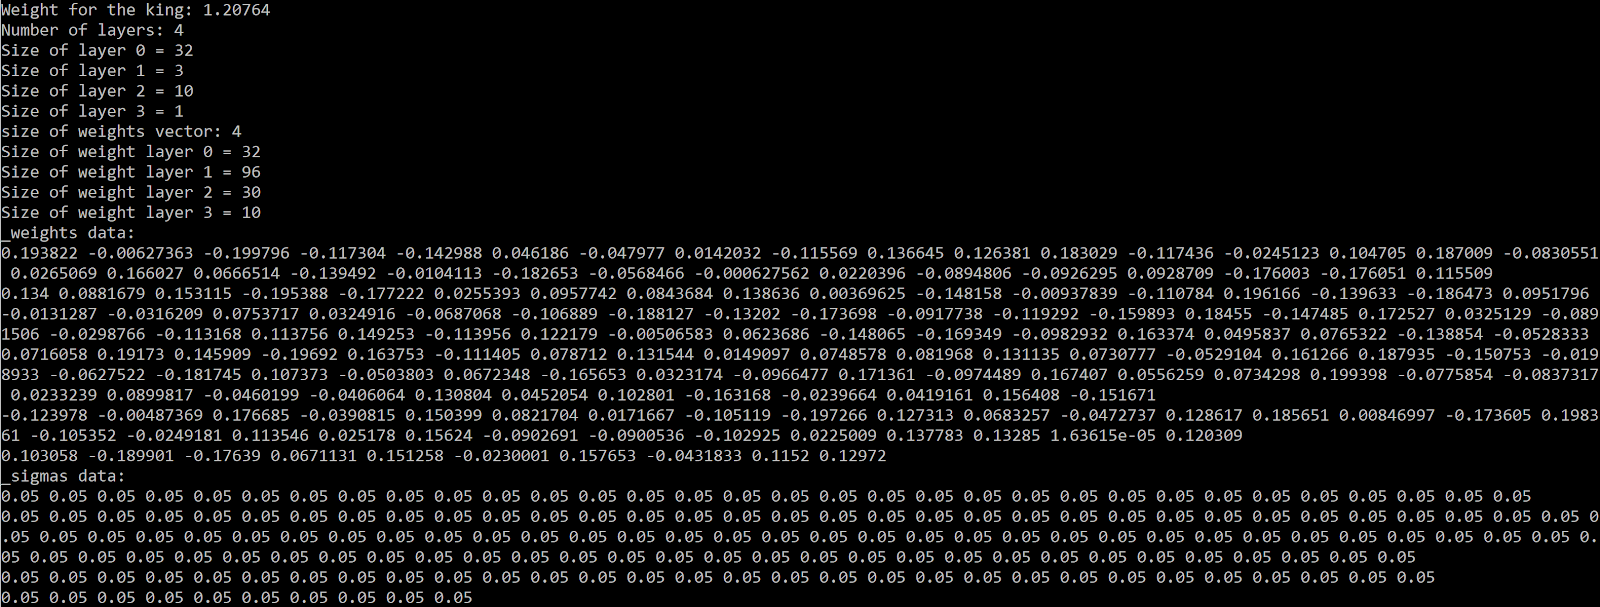
\includegraphics[width=\linewidth]{images/3-10-1-before.png}
    \caption{values before}
    \label{fig:3-10-1-before}
\end{figure}

\begin{figure}
    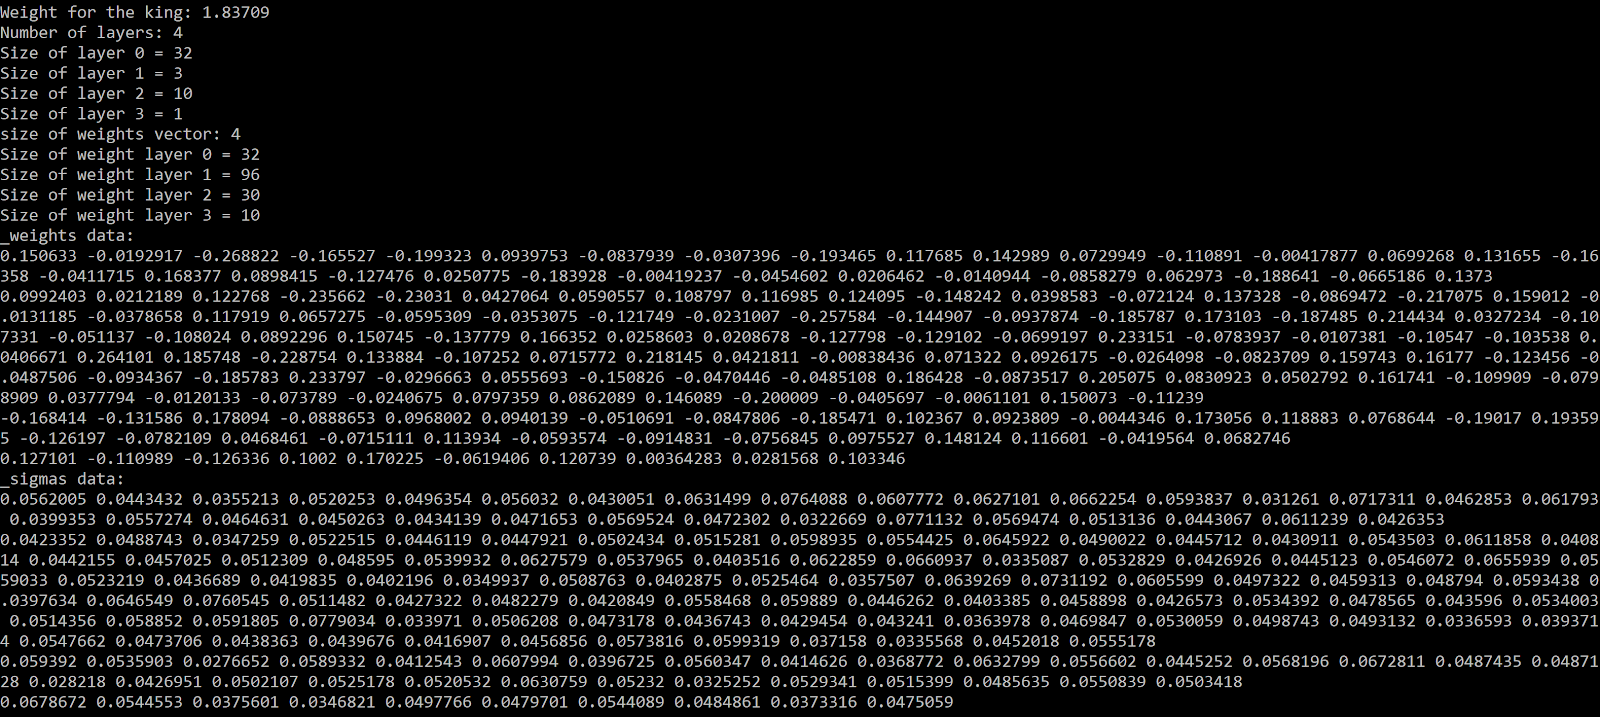
\includegraphics[width=\linewidth]{images/3-10-1-after.png}
    \caption{values after}
    \label{fig:3-10-1-after}
\end{figure}


\begin{figure}
    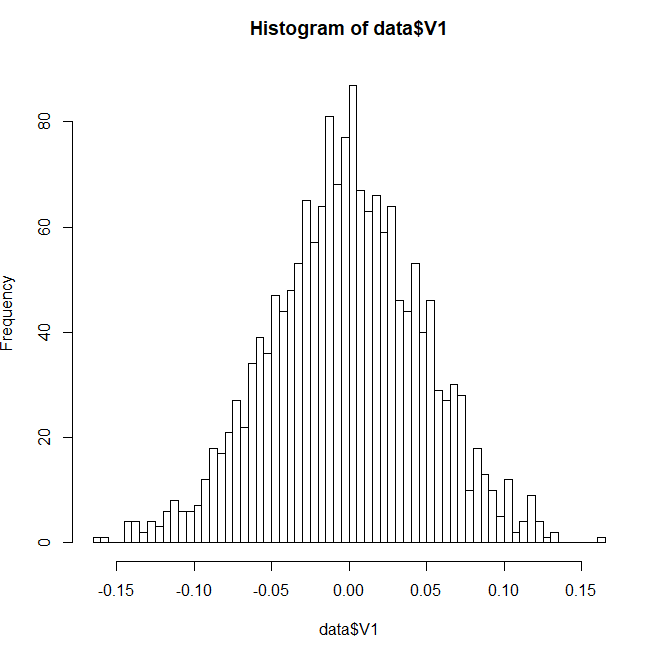
\includegraphics[width=\linewidth]{images/gaussian-1.png}
    \caption{histogram of Gaussian numbers used for evolution}
    \label{fig:gaussian-1}
\end{figure}

\begin{figure}
    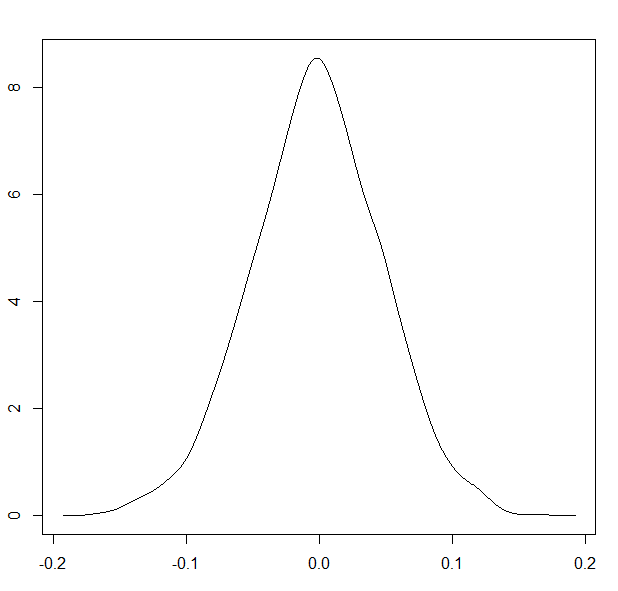
\includegraphics[width=\linewidth]{images/gaussian-2.png}
    \caption{histogram of 1000 Gaussian numbers}
    \label{fig:gaussian-2}
\end{figure}


\end{document}
